\documentclass[fontsize=12pt,paper=a4,twoside,bibtotoc,idxtotoc,
liststotoc,pagesize,BCOR1.2cm,DIV15,chapterprefix,pagesize=pdftex]{scrbook}

%\usepackage[utf8x]{inputenc}
\usepackage[ngerman]{babel}
\usepackage{amsmath}
\usepackage{amssymb}
\usepackage{dsfont}
\usepackage{textcomp}
\usepackage{stmaryrd}
\usepackage{graphicx}
\usepackage{xcolor}

\title{Einführung in Sage}
\author{Dr.Jochen Schulz}
\date{10-10-11}


%\usepackage{fontspec,xunicode}
% %\usepackage{polyglossia}
%\setdefaultlanguage[spelling=new, latesthyphen=true]{german}
%\setsansfont{DejaVu Sans}
%\setsansfont{Verdana}
%\setsansfont{Arial}
%\setromanfont[Mapping=tex-text]{Linux Libertine}
%\setsansfont[Mapping=tex-text]{Myriad Pro}
%\setmonofont[Mapping=tex-text]{Courier New}

%\setsansfont{Linux Biolinum}

\usepackage[ngerman]{babel}
\selectlanguage{ngerman}

%
% math/symbols
%
\usepackage{amssymb}
\usepackage{amsthm}
% \usepackage{latexsym}
\usepackage{amsmath}
%\usepackage{amsxtra} %Weitere Extrasymbole
%\usepackage{empheq} %Gleichungen hervorheben
%\usepackage{bm}
 %\bm{A} Boldface im Mathemodus
\usepackage{fontspec,xunicode,xltxtra}

\usepackage{multimedia}
%\usepackage{tikz}

\usepackage{cellspace}
\setlength{\cellspacetoplimit}{2pt}
\setlength{\cellspacebottomlimit}{2pt}

%%%%%%%%%%%%%%%%%% Fuer Frames [fragile]-Option verwenden!
%Programm-Listing
%%%%%%%%%%%%%%%%%%
%Listingsumgebung fuer verbatim
%Grauhinterlegeter Text
%Automatischer Zeilenumbruch ist aktiviert
%\usepackage{listings}
\usepackage[framed]{mcode}
%\usepackage{mcode}
% This command allows you to typeset syntax highlighted Matlab
% code ``inline''.
% mcode fuer matlab

\definecolor{lgray}{gray}{0.80}
\definecolor{gray}{gray}{0.3}
\definecolor{darkgreen}{rgb}{0,0.4,0}
\definecolor{darkblue}{rgb}{0,0,0.8}
\definecolor{key}{rgb}{0,0.5,0} 
\definecolor{NU0}{RGB}{68,85,136} % #458
\definecolor{KW3}{RGB}{85,68,136}
\definecolor{KW4}{RGB}{153,0,0}
\definecolor{dred}{RGB}{221,17,68} % #d14
\definecolor{BG}{RGB}{240,240,240}
%\lstset{backgroundcolor=\color{lgray}, frame=single, basicstyle=\ttfamily, breaklines=true}
%\lstnewenvironment{sage}{\lstset{,language=python, keywordstyle=color{blue},    commentstyle=color{green}, emphstyle=\color{red}, %frame=single, stringstyle=\color{red}, basicstyle=\ttfamily, ,mathescape =true,escapechar=§}}{}

\lstdefinelanguage{fooHaskell} {%
  basicstyle=\footnotesize\ttfamily,%
  commentstyle=\slshape\color{gray},%
  keywordstyle=\bfseries,%\color{KW4},
  breaklines=true,
  sensitive=true,
  xleftmargin=1pc,
  emph={[1]
    FilePath,IOError,abs,acos,acosh,all,and,any,appendFile,approxRational,asTypeOf,asin,
    asinh,atan,atan2,atanh,basicIORun,break,catch,ceiling,chr,compare,concat,concatMap,
    const,cos,cosh,curry,cycle,decodeFloat,denominator,digitToInt,div,divMod,drop,
    dropWhile,either,elem,encodeFloat,enumFrom,enumFromThen,enumFromThenTo,enumFromTo,
    error,even,exp,exponent,fail,filter,flip,floatDigits,floatRadix,floatRange,floor,
    fmap,foldl,foldl1,foldr,foldr1,fromDouble,fromEnum,fromInt,fromInteger,fromIntegral,
    fromRational,fst,gcd,getChar,getContents,getLine,head,id,inRange,index,init,intToDigit,
    interact,ioError,isAlpha,isAlphaNum,isAscii,isControl,isDenormalized,isDigit,isHexDigit,
    isIEEE,isInfinite,isLower,isNaN,isNegativeZero,isOctDigit,isPrint,isSpace,isUpper,iterate,
    last,lcm,length,lex,lexDigits,lexLitChar,lines,log,logBase,lookup,map,mapM,mapM_,max,
    maxBound,maximum,maybe,min,minBound,minimum,mod,negate,not,notElem,null,numerator,odd,
    or,ord,otherwise,pi,pred,primExitWith,print,product,properFraction,putChar,putStr,putStrLn,quot,
    quotRem,range,rangeSize,read,readDec,readFile,readFloat,readHex,readIO,readInt,readList,readLitChar,
    readLn,readOct,readParen,readSigned,reads,readsPrec,realToFrac,recip,rem,repeat,replicate,return,
    reverse,round,scaleFloat,scanl,scanl1,scanr,scanr1,seq,sequence,sequence_,show,showChar,showInt,
    showList,showLitChar,showParen,showSigned,showString,shows,showsPrec,significand,signum,sin,
    sinh,snd,span,splitAt,sqrt,subtract,succ,sum,tail,take,takeWhile,tan,tanh,threadToIOResult,toEnum,
    toInt,toInteger,toLower,toRational,toUpper,truncate,uncurry,undefined,unlines,until,unwords,unzip,
    unzip3,userError,words,writeFile,zip,zip3,zipWith,zipWith3,listArray,doParse
  },%
  emphstyle={[1]\color{NU0}},%
  emph={[2]
    Bool,Char,Double,Either,Float,IO,Integer,Int,Maybe,Ordering,Rational,Ratio,ReadS,Show,ShowS,String,
    Word8,InPacket
  },%
  emphstyle={[2]\bfseries\color{KW4}},%
  emph={[3]
    case,class,data,deriving,do,else,if,import,in,infixl,infixr,instance,let,
    module,of,primitive,then,type,where
  },
  emphstyle={[3]\color{darkblue}},
  emph={[4]
    quot,rem,div,mod,elem,notElem,seq
  },
  emphstyle={[4]\color{NU0}\bfseries},
  emph={[5]
    EQ,False,GT,Just,LT,Left,Nothing,Right,True,Show,Eq,Ord,Num
  },
  emphstyle={[5]\color{KW4}\bfseries},
  morestring=[b]",%
  morestring=[b]',%
  stringstyle=\color{darkgreen},%
  showstringspaces=false
}
\lstnewenvironment{hs}
{\lstset{language=fooHaskell,backgroundcolor=\color{BG}}}
{\smallskip}
\newcommand{\ihs}[1]{\lstset{language=fooHaskell,basicstyle=\color[gray]{0.6}}\lstinline|#1|}


\lstdefinelanguage{fooMatlab} {%
backgroundcolor=\color[gray]{0.9},
breaklines=true,
basicstyle=\ttfamily\small,
%otherkeywords={ =},
%keywordstyle=\color{blue},
%stringstyle=\color{darkgreen},
showstringspaces=false,
%emph={for, while, if, elif, else, not, and, or, printf, break, continue, return, end, function},
%emphstyle=\color{blue},
%emph={[2]True, False, None, self, NaN, NULL},
%emphstyle=[2]\color{key},
%emph={[3]from, import, as},
%emphstyle=[3]\color{blue},
%upquote=true,
%morecomment=[s]{"""}{"""},
%commentstyle=\color{gray}\slshape,
%framexleftmargin=1mm, framextopmargin=1mm, 
%title=\tiny matlab,
frame=single,
%mathescape =true,
%escapechar=§
}
\newcommand{\imatlab}[1]{\lstset{language=fooMatlab,basicstyle=\color[gray]{0.6}}\lstinline|#1|}
\lstnewenvironment{matlab}[1][]{\lstset{language=fooMatlab,xleftmargin=0.2cm,frame=none,backgroundcolor=\color{white},basicstyle=\color{darkblue}\ttfamily\small,#1}}{} 
\lstnewenvironment{matlabin}[1][]{\lstset{language=fooMatlab,#1}}{} 
\newcommand{\matinput}[1]{\lstset{language=fooMatlab}\lstinputlisting{#1}}

\lstdefinelanguage{fooPython} {%
language=python,
backgroundcolor=\color[gray]{0.7},
breaklines=true,
basicstyle=\ttfamily\small,
%otherkeywords={ =},
keywordstyle=\color{blue},
stringstyle=\color{darkgreen},
morestring=[b]",%
morestring=[b]',%
showstringspaces=false,
emph={class, pass, in, for, while, if, is, elif, else, not, and, or,
def, print, exec, break, continue, return, import, from, lambda, null},
emphstyle=\color{blue},
emph={[2]True, False, None, self},
emphstyle=[2]\color{key},
emph={[3]from, import, as},
emphstyle=[3]\color{blue},
upquote=true,
morecomment=[s]{"""}{"""},
comment=[l]{\#},
commentstyle=\color{gray},
%framexleftmargin=1mm, framextopmargin=1mm, 
%title=\tiny python,
%caption=python,
frame=single
%frameround=tttt,
%mathescape =true,
%escapechar=§
}

\newcommand{\pyinput}[1]{\lstset{language=fooPython}\lstinputlisting{#1}}
\newcommand{\isage}[1]{{\lstset{language=fooPython,basicstyle=\color[gray]{0.3}}\lstinline|#1|}}

\lstnewenvironment{pyout}[1][]{\lstset{language=fooPython,xleftmargin=0.2cm,frame=none,backgroundcolor=\color{white},basicstyle=\color{darkblue}\ttfamily\small,#1}}{}
\lstnewenvironment{pyin}[1][]{\lstset{language=fooPython,#1}}{}
\lstnewenvironment{sageout}[1][]{\lstset{language=fooPython,xleftmargin=0.2cm,frame=none,backgroundcolor=\color{white},basicstyle=\color{darkblue}\ttfamily\small,#1}}{}
\lstnewenvironment{sagein}[1][]{\lstset{language=fooPython,#1}}{}

%\usepackage{caption}
%\DeclareCaptionFont{white}{ \color{white} }
%\DeclareCaptionFormat{listing}{
%  \colorbox[cmyk]{0.43, 0.35, 0.35,0.01 }{
%      \parbox{\textwidth}{\hspace{15pt}#1#2#3}
%        }
%        }
%        \captionsetup[lstlisting]{ format=listing, labelfont=white, textfont=white, singlelinecheck=false, margin=0pt, font={bf,footnotesize} }


\usepackage{mydef}
%\usepackage{cmap} % you can search in the pdf for umlauts and ligatures
\usepackage{colonequals} %corrects the definition-symbols \colonequals (besides others)

\usepackage{ifthen}

%%%%%%%%%%%%%%%%%%%
%Neue Definitionen
%%%%%%%%%%%%%%%%%%%

%Newcommands
\newcommand{\Fun}[1]{\mathcal{#1}}      %Mathcal fuer Funktoren
\newcommand{\field}[1]{\mathbb{#1}}     %Grundkoerper ?? in mathds

\newcommand{\A}{\field{A}}              %Affines A
\newcommand{\Fp}{\field{F}_{\!p}}       %Endlicher Koerper mit p Elementen
\newcommand{\Fq}{\field{F}_{\!q}}       %Endlicher Koerper mit q Elementen
\newcommand{\Ga}{\field{G}_{a}}         %Add Gruppenschema
\newcommand{\K}{\field{K}}              %Generischer Koerper 
\newcommand{\N}{\field{N}}              %Nat Zahlen
\newcommand{\Pj}{\field{P}}             %Projektives P
\newcommand{\R}{\field{R}} 		%Reelle Zahlen
\newcommand{\Q}{\field{Q}}              %Rationale Zahlen  
\newcommand{\Qt}{\field{H}}             %Quaternionen 
\newcommand{\V}{\field{V}}              %Vektorbuendel V
\newcommand{\Z}{\field{Z}}              %Ganze Zahlen
\DeclareMathOperator{\Real}{Re}

\newcommand{\fdg}{\;|\;}                 %fuer die gilt

%Operatoren
\DeclareMathOperator{\Abb}{Abb}
%\usepackage{sagetex}


%
% Aufgaben
%
\parindent0cm % Abs�tze nicht einr�cken 
% Definieren einer neuen Farbe
\definecolor{light-gray}{gray}{.9}

\newcounter{zaehler}     % neuen Z�hler einf�hren
\newenvironment{aufgn}[2][0]
%---- Header
{\begin{samepage}%
%\colorbox{light-gray}{%                         % Box in gray
% \makebox[\textwidth]{%                           % Box in linewidth
%\textbf{Aufgabe \arabic{zaehler} } }\hspace{-\textwidth}\makebox[\textwidth]{\hfill #1 Punkte} }\\[0.05cm]       % Header
\dotfill\\
{\large\textbf{Aufgabe \arabic{zaehler} \ifthenelse{ \equal{#2}{} }{}{: \emph{ #2 } }}\ifthenelse{-1=#1}{(testierbar)}{}\ifthenelse{0=#1 \or -1=#1}{}{\hfill #1 Punkte} }\\[0.4cm]
%{\large\textbf{Exercise \arabic{zaehler}  #2 }\ifthenelse{-1=#1}{(testierbar)}{}\ifthenelse{0=#1 \or -1=#1}{}{\hfill #1 Punkte} }\\[0.4cm]
\begin{minipage}{\textwidth}%
}%
%-----  foot
{\end{minipage}\nopagebreak%\begin{minipage}{1cm} \end{minipage}
%\\ 
%\begin{minipage}{0.1cm} \end{minipage} 
%\hrulefill \begin{minipage}{1cm} \end{minipage}\\[1cm]  
\stepcounter{zaehler}                           % increase counter
\end{samepage}%
\\%
\bigskip%
}


\newenvironment{aufg}[1][0]
%---- Header
{\begin{samepage}%
\refstepcounter{zaehler}% increase counter
%\colorbox{light-gray}{%                         % Box in gray
% \makebox[\textwidth]{%                           % Box in linewidth
%\textbf{Aufgabe \arabic{zaehler} } }\hspace{-\textwidth}\makebox[\textwidth]{\hfill #1 Punkte} }\\[0.05cm]       % Header
\dotfill\\
{\large\textbf{Aufgabe \arabic{zaehler} }\ifthenelse{-1=#1}{(testierbar)}{}\ifthenelse{0=#1 \or -1=#1}{}{\hfill #1 Punkte} }\\[0.4cm]
\begin{minipage}{\textwidth}%
}%
%-----  foot
{\end{minipage}\nopagebreak%\begin{minipage}{1cm} \end{minipage}
%\\ 
%\begin{minipage}{0.1cm} \end{minipage} 
%\hrulefill \begin{minipage}{1cm} \end{minipage}\\[1cm]  
\end{samepage}%
\\%
\bigskip%
}

\begin{document}
\maketitle
\tableofcontents

%%%%%%%%%%%%%%%%%%%%%%%%%%%%%%%%%%%%%%
\chapter{}
\section{Einleitung}
\subsection{Was ist Sage?}
%%%%%%%%%%%%%%%%%%%%%%%%%%%%%%%%%%%%%%

Sage ist ein pythonbasiertes, objektorientiertes Open-source (GPL) Mathematik Software System, dass es seit dem 24. Februar 2005 gibt.
In Sage findet man eine Alternative zu den 4 M's: Magma, Maple, Mathematica, Matlab.\newline
Das (Haupt-)Interface ist der Browser, dennoch besitzt Sage Frontends für viele externe Software.\newline
Zu den Stärken von Sage zählt sicherlich, dass es viele andere CAS und Libraries unter einer einheitlichen Oberfl\"ache vereint 
(so z.B. Maxima, Pari, GAP, R, Magma, ...), sowie durch Python eine sehr mächtige Programmiersprache als Grundlage hat. Desweiteren 
ist der Source Code offen, es gibt ein umfangreiches Hilfesystem sowie viele freie Materialien im Internet.\newline
Wie alles, so hat auch Sage trotz seiner vielen Stärken auch Schwächen, so ist der Befehlsumfang nicht so mächtig, wie der von Maple,Mthematica 
oder Matlab; außerdem fehlt eine standalone Entwicklungsumgebung. Als Alternative zum Webinterface findet sich Cantor.

%%%%%%%%%%%%%%%%%%%%%%%%%%%%%%%%%%%%%%
\subsubsection{Vorab:}
%%%%%%%%%%%%%%%%%%%%%%%%%%%%%%%%%%%%%%

Sage incl. online Testversion und gratis Download sowie einigen anderen Features findet sich unter http://www.sagemath.org/.\newline
Hier ein paar grundlegende Tipps, Tricks und Dinge, die einfach beherzigt werden sollten:\newline
\begin{itemize}
 \item Mehrere Befehle in einer Zeile durch ; trennen. 
 \item Bei Eingaben, die über mehrere Zeilen gehen, kann ein
  Zeilenumbruch durch <ENTER> erreicht werden.
 \item Das Auswerten eines Blocks erfolgt mit {\color{blue} \verb~<SHIFT>+<ENTER>~}.
 \item Ein neues Eingabefeld erhält man durch klicken auf den blauen, horizontalen Balken
 \item {\color{blue} \isage{_} } refenziert die letzte Ausgabe.
 \item Löschen aller eigenen Variablen und Zurücksetzen auf den Anfangsstatus: {\color{blue} \isage{reset()}}
%\item Anzeigen aller definierten Variablen: {\color{blue} anames(All)}
%\item Anzeigen aller selbst definierten Variablen: {\color{blue} anames(All,User)}
 \item Das Feld aktivieren von \emph{Typeset} lässt alle Ausgaben von \LaTeX{} rendern.
%\item profiler und debugger -> commandline
 \item Html- und/oder \LaTeX-Dokumentation:{\color{blue} \verb~<SHIFT>+<KLICK>~ }auf den blauen Balken
%\item Publish: Im Notebook kann durch klicken des \alert{Publish}-Reiters das Notebook für alle offen gelegt werden. 
%\item Unter dem Menupunkt \alert{File} kann man 
 \item {\color{blue} Autocompletion :} mit der {\color{blue} \verb~<TAB>~}-Taste erhält man alle möglichen Funktions- und/oder Variablen-Namen im gegebenen Kontext.\\
  Dies gilt insbesondere auch für Objektfunktionen (\isage{object.function()})
 \item {\color{blue} \isage{<command>?} :} gibt ausführliche Hilfe zu \isage{command} an.
 \item {\color{blue} \isage{help(<command>)} :} öffnet ein Hilfefenster zu \isage{command}.
 \item online Dokumentation:
  \begin{itemize}
   \item Sage: http://www.sagemath.org/doc/index.html
   \item Python: http://docs.python.org/
  \end{itemize}
\end{itemize}
\newpage

%%%%%%%%%%%%%%%%%%%%%%%%%%%%%%%%%%%%%%
\subsection{Überblick}
%%%%%%%%%%%%%%%%%%%%%%%%%%%%%%%%%%%%%%

Als Einstieg und kleine Motivation, wofür man Sage einsetzen kann, wollen wir erst einmal ein paar grundlegende Operationen 
vorstellen:
\begin{itemize}
 \item Deklarieren von Variablen mir \isage{var()}, z.B.{\verb~var('a')~} 
 \item Definieren von Variablen mit {\color{blue}'='}, z.B. {\verb~a=3~} 
 \item Definieren von Funktionen mit{\color{blue} '='}, z.B. {\verb~f(x) = x^2 - 6*x~}
 \item Grenzwertbestimmung: {\color{blue}   \verb~f.limit(x=1, dir='<plus|minus>')~}
 \item Bilden von Ableitungen {\color{blue} \verb~f.differentiate(x)~}
 \item Lösen von Gleichungen: {\color{blue} \verb~solve( f(x)==0, x)~}
 \item Berechnen numerischer Approximationen: {\color{blue} \verb~float(f(sqrt(3)+ 4))~}
 \item Plotten einer Funktion: {\color{blue} \verb~plot(sin,(0,4))~}
 \item symbolisch Integrieren: {\color{blue} \verb~integrate(f,x)~}
 \item numerisch Integrieren: {\color{blue} \verb~integrate(f,x,a,b)~}
 \item Faktorisieren: {\color{blue} \verb~expand(f)~}
 \item Sortieren: {\color{blue} \verb~f.collect(x)~}
 \item Partialbruchzerlegung: {\color{blue} \verb~f.partial_fraction()~}
 \item vollständiges Vereinfachen: {\color{blue} \verb~f.full_simplify()~}
 \item Vereinfachen mit radicals: {\color{blue} \verb~f.radical_simplify()~}
 \item Matrix eingeben: {\color{blue} \verb~matrix([ [z1s1,z1s2],[z2s1,z2s2] ])~}
 \item Vektor eingeben: {\color{blue} \verb~vector([a,b,c])~}
 \item LGS lösen: {\color{blue} \verb~A\b~}
 \item Matrixoperationen: {\color{blue} \verb~A+B,A-B,A*B~}
 \item Matrix invertieren: {\color{blue} \verb~A^(-1); A.inverse()~}
 \item Substitutieren: {\color{blue} \verb~f.subs(k=2)~}
\end{itemize}
Hiermit stehen uns nun einige Türen offen und wir wollen uns an ein paar Beispielen der Sagewelt nähern:\newpage

%%%%%%%%%%%%%%%%%%%%%%%%%%%%%%%%%%%%%%
\subsubsection{1. Kurvendiskussion}
%%%%%%%%%%%%%%%%%%%%%%%%%%%%%%%%%%%%%%

Wir wollen eine handelsübliche Kurvendiskussion führen. Dazu betrachten wir die durch die reelle Zahl $a$ parametrisierte 
Funktionenschar:
\[ 
f: x \quad \mapsto \quad \frac{2x^2-20x+42}{x-1}+a, \quad
a \in \mathbb{R} 
\]
Wie bekommen wir nun diese Aufgabe mittels Sage gelöst? Zuerst sollten wir diese Funktionenschar wohl Sage ``erklären'', 
um weiter mit ihr arbeiten zu können. Dies geschiet, indem wir zuerst die Variable $a$ und anschließend die Funktion selbst 
deklarieren:\newline
\begin{sagein}
var('a')
f(x) = (2*x^2-20*x +42)/(x-1)+a;f
\end{sagein}
\textbf{Bemerkung:} Die Multiplikationszeichen dürfen NICHT weggelassen werden.\newline
Wir erhalten als Antwort\newline
\begin{sage}
  x |--> a + 2*(x^2 - 10*x + 21)/(x - 1)
\end{sage}
\textbf{Bemerkung:} Es findet keine Ausgabe statt, wenn wir in unserer Eingabe ;f weglassen.\newline
Wir möchten nun herausfinden, ob unsere Funktion Polstellen besitzt; dazu benutzen wir den limit Befehl:\newline
\begin{sagein}
f.limit(x=1, dir='minus')
\end{sagein}
\begin{sage}
  x |--> -Infinity
\end{sage}
\begin{sagein}
f.limit(x=1, dir='plus') 
\end{sagein}
\begin{sage}
  x |--> +Infinity
\end{sage}
Wir sehen nun, dass unsere Funktion f an der Stelle x=1 einen Pol hat. Wir verfahren weiter mit der Suche nach Nullstellen 
und wenden dafür den solve Befehl an:\newline
\begin{sagein}
solve(f==0,x)
\end{sagein}
\begin{sage}
[x == -1/4*a - 1/4*sqrt(a^2 - 32*a + 64) + 5, x == -1/4*a + 1/4*sqrt(a^2 - 32*a + 64) + 5]
\end{sage}
Wir haben nun 2 Nullstellen gefunden und stellen uns sogleich die Frage nach der Ableitunge von f, die wir über den 
differentiate Befehl erhalten:\newline
\begin{sagein}
f.differentiate(x)
\end{sagein}
\begin{sage} 
x |--> 4*(x - 5)/(x - 1) - 2*(x^2 - 10*x + 21)/(x - 1)^2
\end{sage}
Da unsere Funktion offenbar eine Ableitung besitzt, interessiert uns, ob und, wenn ja, wo f Extrema besitzt sowie die Antwort 
auf die Frage, ob es sich um Minima oder MAxima handelt:\newline
\begin{sagein}
maxi = solve(f.differentiate(x)==0,x); maxi
\end{sagein}
\begin{sage}
[x == -2*sqrt(3) + 1, x == 2*sqrt(3) + 1]
\end{sage}
\begin{sagein}
float( ((f.diff(x)).diff(x))(maxi[0].rhs()) )
\end{sagein}
\begin{sage}
-1.1547005383792501
\end{sage}
\begin{sagein}
float( ((f.diff(x)).diff(x))(maxi[1].rhs()) )
\end{sagein}
\begin{sage}
1.1547005383792515
\end{sage}
Wir erkennen die Existenz zweier Extremstellen, von denen eines ein Maximum, das andere ein Minimum ist.\newline
\textbf{Bemerkung:} Als ``Speicherplatz'' der Nullstellen von f' besitzt maxi zwei Werte- diese werden mit maxi[0].rhs() 
bzw maxi[1].rhs() angesprochen.\newline
Ohne den float() Befehl sähe die Ausgabe im ersten Fall so aus:
\begin{sagein}
-1/18*((2*sqrt(3) - 1)^2 + 20*sqrt(3) + 11)*sqrt(3) + 2/3*sqrt(3) + 8/3
\end{sagein}
und wäre somit unbrauchbar, um direkt ein Maximum oder Minimum erkennen zu können.\newline
Zuletzt betrachten wir noch das Verhalten am Rande:\newline
\begin{sagein}
f.limit(x=oo); f.limit(x=-oo)
\end{sagein}
\begin{sage}
x |--> +Infinity
x |--> -Infinity
\end{sage}
\textbf{Bemerkung:} Wir erkennen, in Sage stellt sich $\infty$ dar via oo, $-\infty$ entspricht offenbar -oo.\newline
Viel interessanter jedoch ist die Tatsache, dass Sage mit jenen ``Werten'' direkt arbeiten zu können scheint.\newline
Zuletzt wollen wir uns mit der grafischen Darstellung einiger Repräsentanten von f auseinandersetzen. Hierzu wollen wir zuerst 3 
jener Repräsentanten deklarieren und diese anschließend mit dem plot Befehl visualisieren:\newline
\begin{sagein}
 f0 = f(x, a=0)
 f1 = f(x, a=-20)
 f2 = f(x, a=20);f0,f1,f2
\end{sagein}
\begin{sage}
(2*(x^2 - 10*x + 21)/(x - 1), 2*(x^2 - 10*x + 21)/(x - 1) - 20, 2*(x^2 - 10*x + 21)/(x - 1) + 20)
\end{sage}
\begin{sagein}
p = plot(f0,detect_poles='show',xmin=0, xmax=10,color='red')
p += plot(f1,detect_poles='show',xmin=0, xmax=10,color='green')
p += plot(f2,detect_poles='show',xmin=0, xmax=10,color='blue'); p.show(ymin=-80, ymax=80)
\end{sagein}
Wir erhalten als Grafikausgabe:
\begin{center}
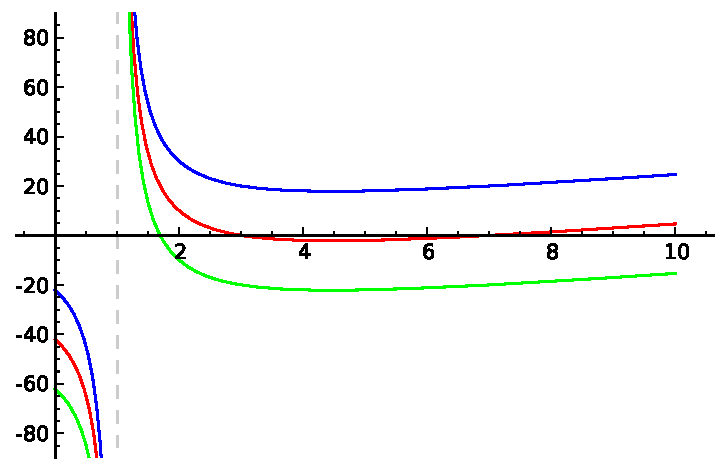
\includegraphics[height=4.5cm]{graphen}
\end{center}\newpage

%%%%%%%%%%%%%%%%%%%%%%%%%%%%%%%%%%%%%%
\subsubsection{2. Symbolisches Rechnen}
%%%%%%%%%%%%%%%%%%%%%%%%%%%%%%%%%%%%%%

Wir wollen uns nun ein wenig mit symbolischem Rechnen vertraut machen; dazu zählt das numerische Lösen von Integralen, 
sicherlich aber auch die Vereinfachung oder die Faktorisierung eines Terms. Wir betrachten einige Beispiele:\newline
Wir möchten gerne das Integral $\int_0^\infty x^4 e^{-x} dx$ numerisch berechnen, dazu benötigen wir lediglich
\begin{sagein}
integrate(x^4*exp(-x),x,0,oo)
\end{sagein}
und erhalten als Ausgabe 
\begin{sage}
  24
\end{sage}.
Wollen wir eine Stammfunktion von $\frac{1+\sin (x)}{1+\cos(x)}$ berechnen, so genügt uns die Deklaration zweier Funktion f
und g wie folgt:
\begin{sagein}
f(x) = (1+sin(x))/(1+cos(x))
g = f.integrate(x);g
\end{sagein}
\begin{sage}
x |--> sin(x)/(cos(x) + 1) - log(cos(x) + 1)
\end{sage}
Die Funktion g sieht eher unschön aus, wir möchten sie daher vereinfachen und benutzen dafür
\begin{sagein}
g.full_simplify()
\end{sagein}
\begin{sage}
x |--> -((cos(x) + 1)*log(cos(x) + 1) - sin(x))/(cos(x) + 1)
\end{sage}
Die Verschönerung hat hier nur bedingt geklappt, aber der Versuch war es wert und oft erhält man wirklich ein schöneres 
Ergebnis als zuvor. Ein wenig effektiver funktioniert es mit ($\frac{e^x -1}{e^{(1/2)x}+1}$)
\begin{sagein}
g = (exp(x)-1)/(exp(x/2)+1)
g.simplify_radical()
\end{sagein}
\begin{sage}
 e^(1/2*x) - 1
\end{sage}
Es gibt noch andere Möglichkeiten, Termen ein schöneres Aussehen zu geben. Betrachten wir den Term
\begin{sage}
x^4 - 10*x^3 + 35*x^2 - 50*x + 24
\end{sage}
und fragen uns: Können wir ihn Faktorisieren? Eine Antwort darauf liefert 
\begin{sagein}
factor(x^4 - 10*x^3 + 35*x^2 - 50*x + 24)
\end{sagein}
\begin{sage}
(x - 4)*(x - 3)*(x - 2)*(x - 1)
\end{sage}
Als kleine Probe können wir die Faktorisierung rückgängig machen:
\begin{sagein}
expand(_)
\end{sagein}
\begin{sage}
x^4 - 10*x^3 + 35*x^2 - 50*x + 24
\end{sage}
\textbf{Bemerkung:} Wir erinnern uns, dass \_ eine Referenz auf die letzte Ausgabe ist.\newline
Wir können Terme Terme auch bzgl. einer Variablen sortieren lassen:\newline
\begin{sagein}
var('b,a')
g = x^2+2*x+b*x^2+sin(x)+a*x
g.collect(x)
\end{sagein}
\begin{sage}
(b + 1)*x^2 + (a + 2)*x + sin(x)
\end{sage}
Zuletzt steht uns hier noch die Partialbruchzerlegung zur Verfügung:\newline
\begin{sagein}
g = x^ 2/( x^ 2- 1)
g.partial_fraction()
\end{sagein}
\begin{sage}
1/2/(x - 1) - 1/2/(x + 1) + 1
\end{sage}
\newpage

%%%%%%%%%%%%%%%%%%%%%%%%%%%%%%%%%%%%%%
\subsubsection{3. Analytische Geometrie und Lineare Algebra}
%%%%%%%%%%%%%%%%%%%%%%%%%%%%%%%%%%%%%%

Wir wollen uns ein wenig mit analytischer Geometrie und linearer Algebra beschäftigen und zu Anfang mal den Schnittpunkt einer Ebene mit einer Geraden 
berechnen. Dazu sei die Ebene E gegeben durch
\[ E: \vec{x}= 
\left ( \begin{array}{c}  2 \\ 1 \\ -1 \end{array} \right) +l 
\left ( \begin{array}{c}  1 \\ -1 \\ -1 \end{array} \right) +m
\left ( \begin{array}{c}  -3 \\ 1 \\ 4 \end{array} \right), \quad l,m
\in \mathbb{R}
\]
und die Gerade g
\[
g: \vec{x}=
\left ( \begin{array}{c}  3 \\ 0 \\ 1 \end{array} \right) +k
\left ( \begin{array}{c}  4 \\ -1 \\ 2 \end{array} \right), \quad k \in \mathbb{R}
\]
Gleichsetzen ergibt: 
\[ 
\left ( \begin{array}{c}  2 \\ 1 \\ -1 \end{array} \right) +l 
\left ( \begin{array}{c}  1 \\ -1 \\ -1 \end{array} \right) +m
\left ( \begin{array}{c}  -3 \\ 1 \\ 4 \end{array} \right) = \left ( \begin{array}{c}  3 \\ 0 \\ 1 \end{array} \right) +k
\left ( \begin{array}{c}  4 \\ -1 \\ 2 \end{array} \right)
\] oder {
\[ 
\underbrace{\left(   
\begin{array} {ccc} 
1 & -3 & -4\\
-1 & 1 & 1 \\
-1 & 4 & -2  
\end{array} \right)}_{\displaystyle =:A} 
\underbrace{\left ( \begin{array}{c}  l \\ m \\ k \end{array}
  \right)}_{\displaystyle =:L} = \underbrace{\left ( \begin{array}{c}  1 \\ -1 \\ 2
  \end{array} \right)}_{\displaystyle =:b}
\] }
oder $A L=b$.
Wir wollen nun lineare Gleichungssysteme (wie dieses) wie gewöhnlich durch MAtrizen beschreiben und via Sage lösen. Dazu benötigen wir ein paar Grundlagen:
\begin{itemize}
\item Definieren der Matrix $A$
\begin{sagein}
A = matrix([[1,-3,-4],[-1,1,1],[-1,4,-2]]); A
\end{sagein}
\begin{sage}
[ 1 -3 -4]
[-1  1  1]
[-1  4 -2]
\end{sage}
\item Definieren des Vektors $b$
\begin{sagein}
b = vector([1,-1,2])
\end{sagein}
\item Lösen von  $A \ L=b$
\begin{sagein}
A.solve_right(b)
\end{sagein}
oder 
\begin{sagein}
A\b
\end{sagein}
ergibt
\begin{sage}
(6/5, 3/5, -2/5)
\end{sage}
\item Einsetzen in die Geradengleichung
\begin{sagein}
x_s = matrix([g1,g2,g3]).subs(k=L[2]); x_s
\end{sagein}
\begin{sage}
[7/5 2/5 1/5]
\end{sage}
\end{itemize}
So haben wir nun recht aufwandsarm den Schnittpunkt der beiden Objekte E und g erhalten. Wir geben noch einen kurzen Ausblick auf weitere 
Matrizenoperationen:\newline
\begin{sagein}
B = matrix([[1,0,0],[0,1,1],[1,1,1]])
A*B; A-B; A+B
\end{sagein}
\begin{sage}
[-3 -7 -7]  [ 0 -3 -4] [ 2 -3 -4]
[ 0  2  2]  [-1  0  0] [-1  2  2]
[-3  2  2]  [-2  3 -3] [ 0  5 -1]
\end{sage}
Berechnen der Inversen (mit Probe)
\begin{sagein}
$A^(-1)$, A*A^(-1)
\end{sagein}
\begin{sage}
[  -2/5 -22/15   1/15]
[  -1/5   -2/5    1/5]
[  -1/5  -1/15  -2/15]

[1 0 0]
[0 1 0]
[0 0 1]
\end{sage}
Wir wollen uns das Ganze mal visualisieren, hierzu bietet uns Sage den 3D plot:
\begin{sagein}
var('l,m'); E1 = 2+l-3*m; E2 = 1-l+m; E3 =-1-l+4*m
p = parametric_plot3d([E1,E2,E3],(l,-2,2),(m,-2,2), color='green', opacity=0.8)
var('k'); g1 = 3+4*k; g2 = -k; g3 = 1+2*k
p += parametric_plot3d( (g1,g2,g3), (k, -3, 3),thickness='3' ) 
p.show()
\end{sagein}
\begin{center}
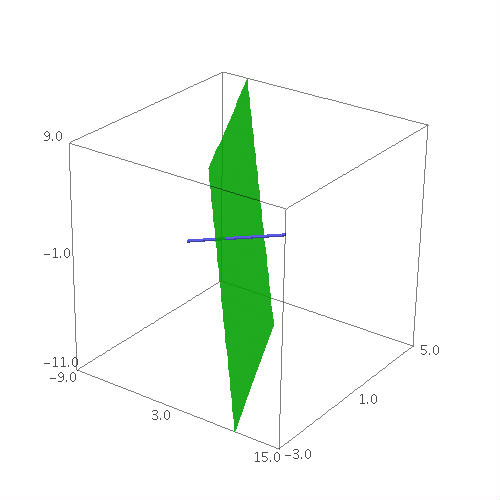
\includegraphics[width=0.7\textwidth]{ebene2}
\end{center}
\textbf{Bemerkung:} In Sage lässt sich der 3D plot drehen.
\newpage

%%%%%%%%%%%%%%%%%%%%%%%%%%%%%%%%%%%%%%
\subsubsection{4. Programmieren}
%%%%%%%%%%%%%%%%%%%%%%%%%%%%%%%%%%%%%%

\begin{itemize}
 \item Wir möchten eine einzeilige Funktion definieren. Dies geschieht via
  \begin{sagein}
  def <name>(<Argumente>) : return <Rueckgabe>
  \end{sagein}
  Beispiel: 
  \begin{sagein}
  def fd(ex) : return diff(ex)
  fd(x^2)
  \end{sagein}
  \begin{sage}
  2*x
  \end{sage}
 \item Wir können Objekte in Listen und Tupeln zusammenfassen:\newline
  Eine \emph{Liste} ist in Sage (und Python) mit \isage{[..,..]} gekennzeichnet
  \begin{sagein}
  liste = [21,22,24,23]
  liste.sort(); liste 
  \end{sagein}
  \begin{sage}
  [21, 22, 23, 24]
  \end{sage}
  Ein \emph{Tuple} ist in Sage (und Python) mit \isage{(..,..)} gekennzeichnet 
  \begin{sagein}
  tuple = (liste[0], liste[2])
  tuple, tuple[0]
  \end{sagein}
  \begin{sage}
  ((21, 24), 21) 
  \end{sage}
  Liste von ganzen Zahlen von \isage{a} bis \isage{b}
  \begin{sagein}
  [a..b] ; range(a,b+1)
  \end{sagein}
 \item Es gibt einzeilige (bedingte) Schleifen:
  \begin{sagein}
  [<expr(var)> for <var> in <range|liste>] 
  [<expr(var)> for <var> in <range|liste> if <expr>] 
  \end{sagein}
  Beispiel:
  \begin{sagein}
  [m^2 for m in [1..5] ]
  \end{sagein}
  \begin{sage}
  [1, 4, 9, 16, 25]
  \end{sage}
  Beispiel mit Abfrage:
  \begin{sagein}
  [m^2 for m in [1..5] if m%2==0]
  \end{sagein}
  \begin{sage}
  [4, 16]
  \end{sage}
\end{itemize}

%%%%%%%%%%%%%%%%%%%%%%%%%%%%%%%%%%%%%%
\subsubsection{6. Zahlentheorie}
%%%%%%%%%%%%%%%%%%%%%%%%%%%%%%%%%%%%%%

Wir sind nun in der Lage, etwas kompliziertere Aufgabenstellungen zu bearbeiten:\newline
1.Die Fermatschen Primzahlen sind gegeben durch $F_n=2^{2^n} +1$. Wir wollen die kleinste dieser Zahlen finden, die keine Primzahl ist. Dazu 
schreiben wir uns ein kleines Programm:
\begin{sagein}
def F(n): return 2^(2^n)+1
[[F(m),is_prime(F(m))] for m in range(1,6)]
\end{sagein}
\begin{sage}
[[5, True], [17, True], [257, True], [65537, True], [4294967297, False]]
\end{sage}
Uns interssieren nun noch die Teiler von $F_5$
\begin{sagein}
divisors(int(F(5)))
\end{sagein}
\begin{sage}
[1, 641, 6700417, 4294967297]
\end{sage}
2. Wir möchten eine Liste der Primzahlen bis 100:
\begin{sagein}
menge = range(1,101)
[m for m in menge if is_prime(m)]
oder filter(is_prime,menge)
\end{sagein}
\begin{sage}
[2, 3, 5, 7, 11, 13, 17, 19, 23, 29, 31, 37, 41, 43, 47, 53, 59, 61, 67, 71, 73, 79, 83, 89, 97]
\end{sage}
3.Die Mersenne Primzahlen sind gegeben durch $2^p-1$, dabei $p$ Primzahl. Wir wollen die Mersenne Primzahlen im Bereich $\leq200$ bestimmen:
\begin{sagein}
menge = range(1,201)
primes = [m for m in menge if is_prime(m)]
[2^m-1 for m in primes if is_prime(2^m-1)]
\end{sagein}
\begin{sage}
[3, 7, 31, 127, 8191, 131071, 524287, 2147483647, 2305843009213693951,
618970019642690137449562111, 162259276829213363391578010288127,
170141183460469231731687303715884105727]
\end{sage}
4.Wir wollen für die Zahlen $\leq1000$ bestimmen, wieviele Zahlen 1,2,3,... Teiler haben:
\begin{sagein}
menge = range(1,1001)
liste = [number_of_divisors(int(m)) for m in menge]
[(i,len([m for m in liste if m==i]))for i in range(1,51)]
\end{sagein}

\begin{sage}
[(1, 1), (2, 168), (3, 11), (4, 292), (5, 3), (6, 110), (7, 2), (8,
180), (9, 8), (10, 22), (11, 0), (12, 97), (13, 0), (14, 5), (15, 4),
...
\end{sage}
Bis hierher haben wir einen kleinen Rundumblick genommen, einige sehr elementare Grundlagen kennengelernt und sind schon recht vertraut mit 
Sage. Vieles von dem, was wir bisher gesehen haben, wird uns wieder begegnen, wenn wir uns weiter mit Sage befassen.
\end{document}